% Comentários Douglas
%  - Rever os objetivos específicos e geral para deixar mais explicativo e fechar melhor o escopo
%  - Materiais antes de métodos
%  - Trabalhos relacionados pode ser melhor explorados
%  - Fraco refereciamento em vários itens do texto
%  - Muitas palavras em inglês
%  - Melhorar requisito funcionais
%  - Falta um texto de suporte do visão geral
%  - Faltam diagramas para suportar a implementação (e não dos testes) junto ou talvez substituir trechos de código

% Comentários Tiago
%  - Destacar melhor características de tempo real: se não injetar nenhuma falta o seu sistema pode falhar?
%  - Destacar que o sistema é de tempo real e qual é o requisito de tempo real
%  - heartbit talvez seja a técnica para atrelar em teste de atender o requisito de tempo real.
%  - Plano de teste alinhados com os requisitos
%  - Diagramas de sequência (ou fluxograma) entre outros para descrever os testes 
%  - Analisar cronograma para realizar os testes

\chapter{Projeto}
\label{cap:proj}

\section{Visão Geral}

Serão implementados mecanismos de tolerância utilizando do FreeRTOS como base, as técnicas implementadas serão discutidas em maior detalhe na \autoref{subsec:algoritmos}. Para a coleta das métricas de eficácia e custo computacional será utilizado um cenário de injeção de falhas lógicas em hardware utilizando do depurador em chip ST-Link, os detalhes da campanha de injeção de falhas são abordados na \autoref{subsec:campanhaInjecao}.

A \autoref{fig:visaoGeral} sumariza a relação entre os principais componentes, as técnicas de tolerância são implementadas como complementos ao FreeRTOS e o processo de injeção é controlado por um computador externo que envia comandos para o depurador em chip com o propósito de simular uma falha.

\begin{figure}[H]
    \centering
    \captionsetup{justification=centering}
    \caption{Principais componentes do projeto}
    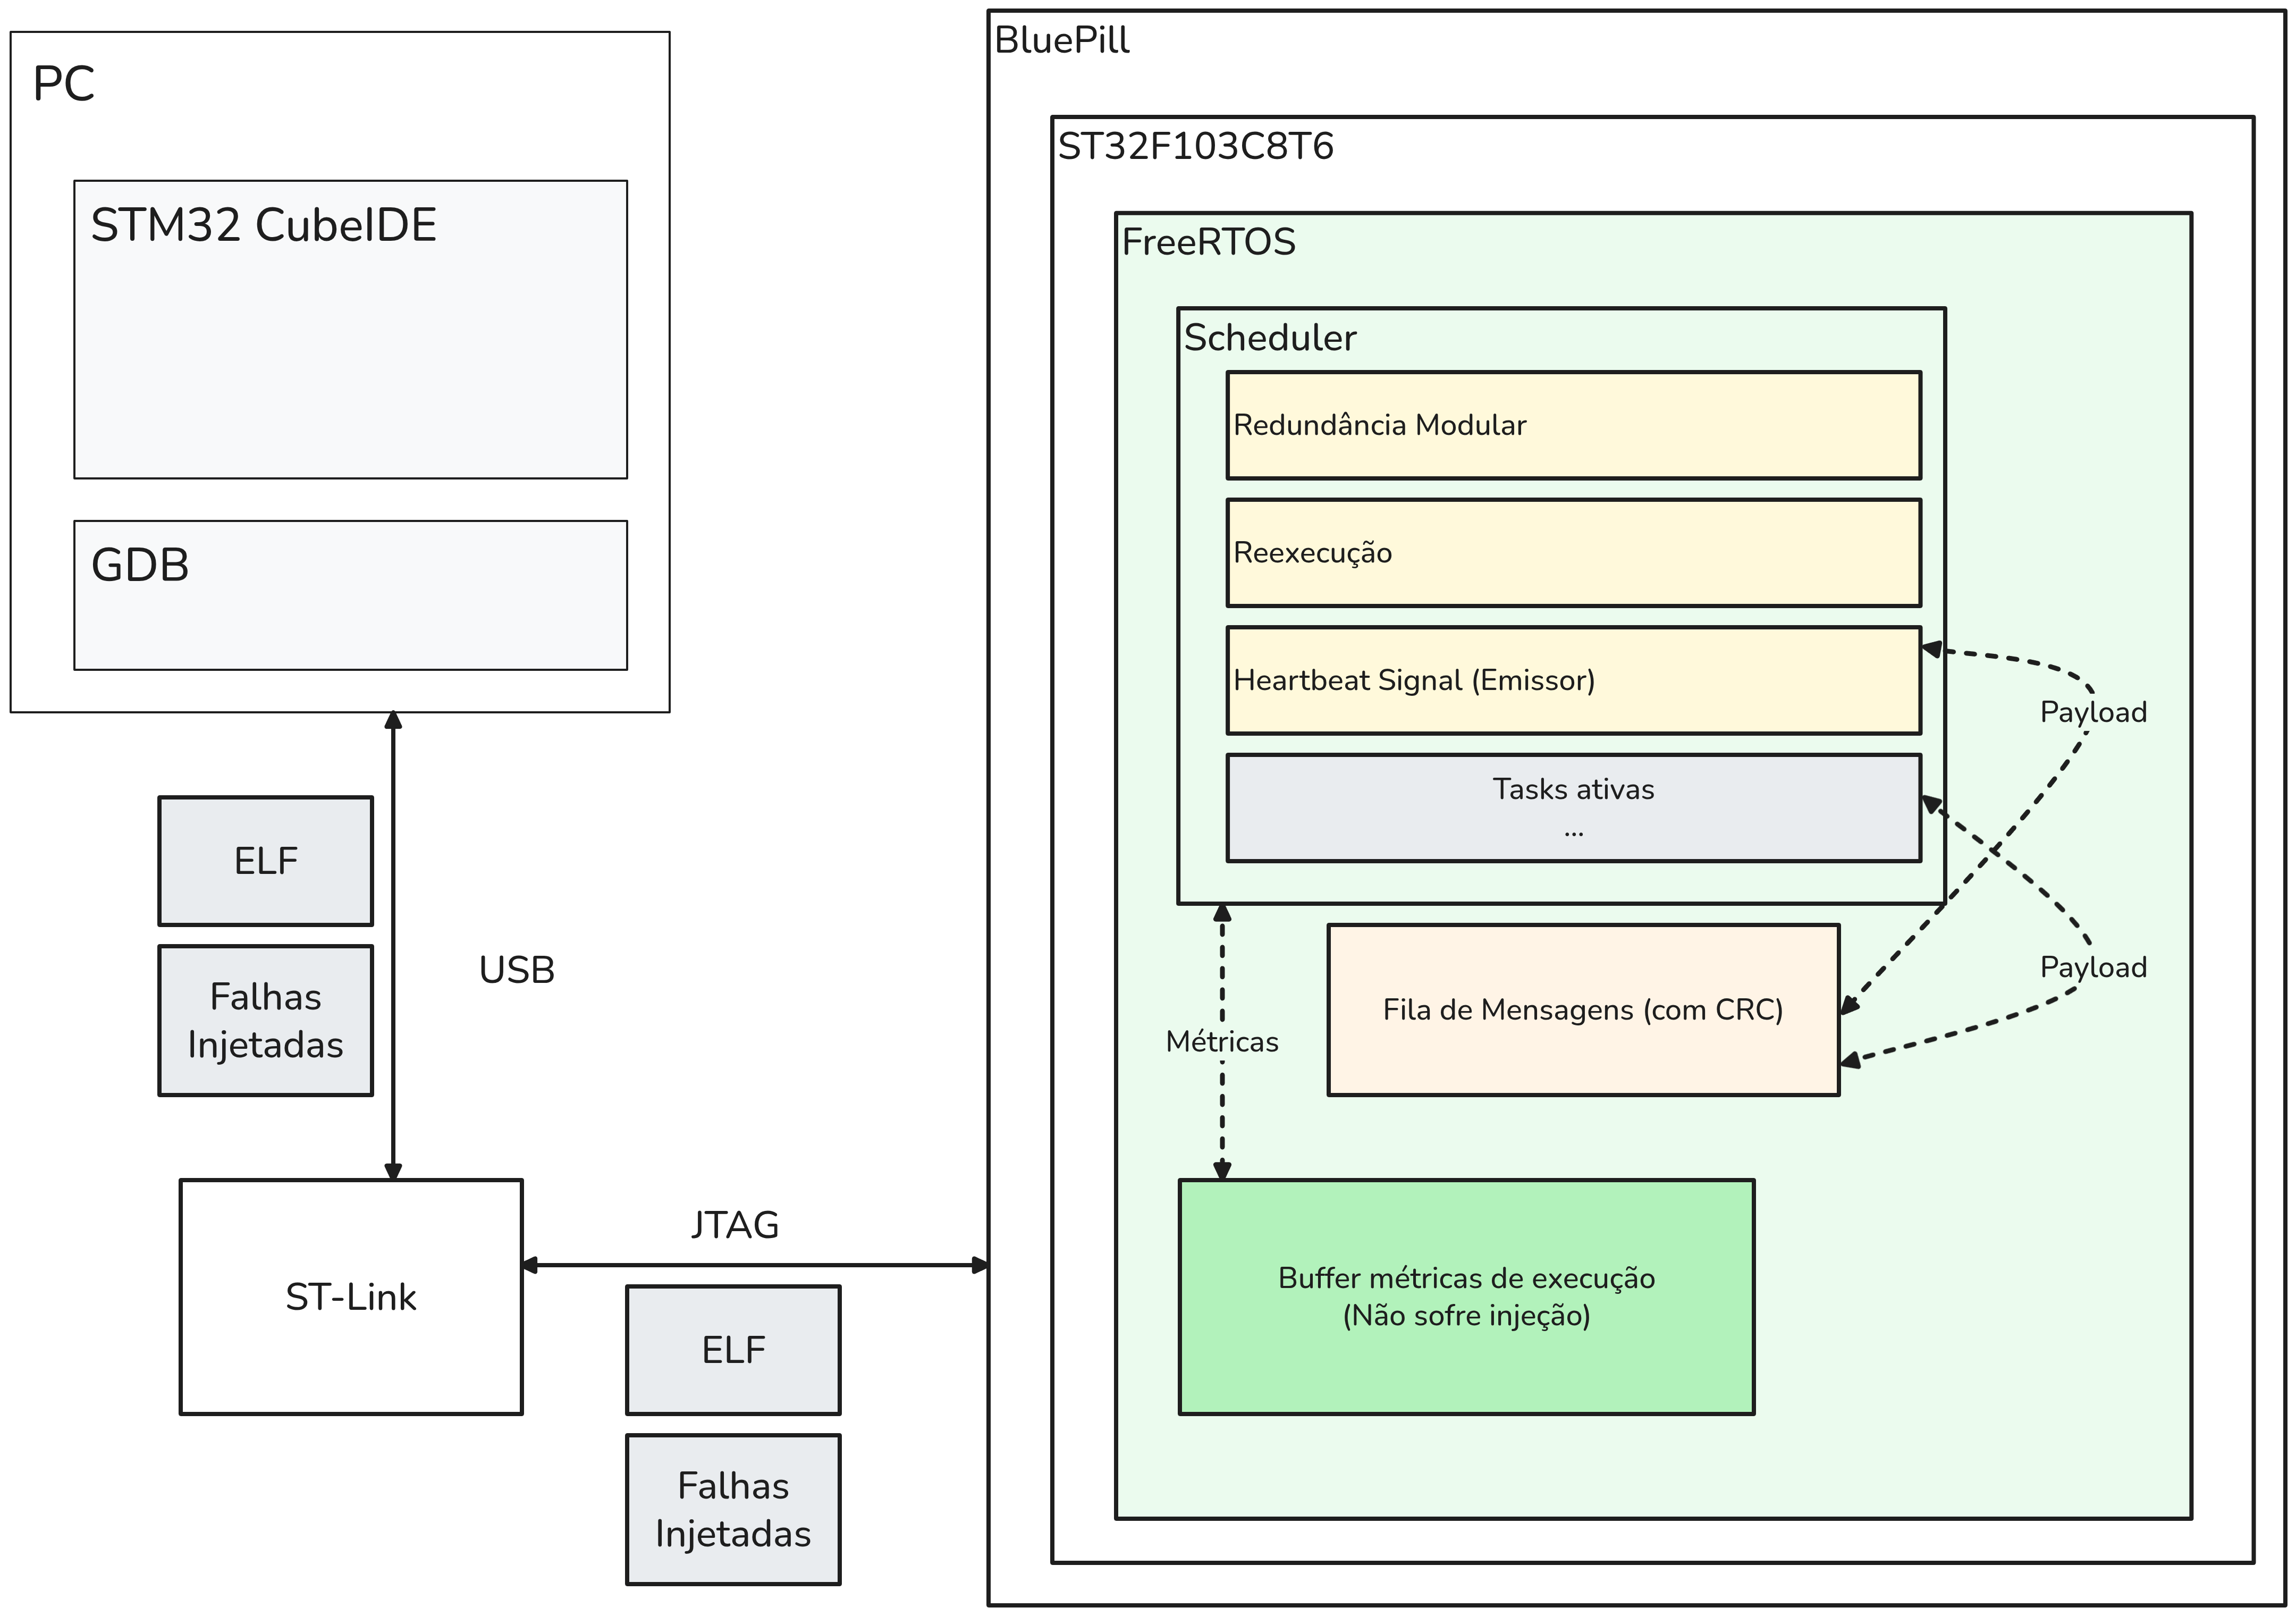
\includegraphics[width=0.97\textwidth]{assets/visao_geral.png}
    \captionsetup{justification=raggedright}
    \caption*{Fonte: Elaborada pelo autor}
    \label{fig:visaoGeral}
\end{figure}

\section{Premissas}

Será partido do ponto que ao menos o processador que executa o escalonador terá registradores de controle (ponteiro de pilha, contador de programa, endereço de retorno) que sejam capazes de mascarar falhas. Apesar de ser possível executar os algoritmos reforçados com análise de fluxo do programa e adicionar redundância aos registradores, isso adiciona um grau a mais de complexidade que foge do escopo do trabalho. Como mencionado na \autoref{sec:trabRel}, a memória fora do banco de registradores pode ser duas ordens de magnitude mais sensível à eventos disruptivos \cite{ReliabilityArmCortexUnderHeavyIons}.

O sistema tentará atingir um critério de Hard Real-Time, isto é, o descumprimento de um prazo de execução será considerado uma falha completa. Prazos de execução podem ser locais à um segmento particular do programa ou globais que correspondem ao programa como um todo ou à um macro processo. A escolha do critério Hard Real-Time também é útil de um ponto de vista da análise pois será possível comparar o custo temporal da aplicação de técnicas em relação ao limite de execução.

Com o fim de reduzir o tamanho do executável e manter o fluxo de mais previsível não serão utilizados mecanismos de exceção com desenrolamento (\textit{unwinding}) da pilha. Também não será utilizado de RTTI (Runtime Type Information). Todos os erros devem portanto ser tratados como valores ou como falhas lógicas.

Necessariamente, é preciso também presumir que testes sintéticos possam ao menos aproximar a performance do mundo real, ou ao menos prever o pior caso possível com grau razoável de acurácia. O uso de testes sintéticos não deve ser um substituto para a medição em uma aplicação real, porém, uma bateria de testes com injeção artificial de falhas pode ser utilizada para verificar as tendências e custos relativos introduzidos, mesmo que não necessariamente reflitam as medidas absolutas do produto final.

Portanto, será assumido que os resultados extraídos de injeção de falhas artificiais, apesar de menos condizentes com os valores absolutos de uma aplicação e não sendo substitutos adequados na fase de aprovação de um produto real, são ao menos capazes para realizar uma análise quanto ao custo proporcional introduzido, e devido à sua facilidade de realização e profundidade de inspeção possível, serão priorizados inicialmente neste projeto.

\section{Metodologia}

\subsection{Materiais}

% TODO: sumarizar, mais diagramas, melhorar coesao deixar um pouco mais segmentado e com conexoes entre os topicos, aqui e em metodos. referenciar as figuras

Será utilizada a linguagem C++ com o compilador GCC (ou Clang), o alvo principal do trabalho será um microcontrolador STM32F103C8T6 "Bluepill" 32-bits da arquitetura ARMv7-M, como visto na \autoref{fig:stm32Bluepill}.

\begin{figure}[H]
    \centering
    \captionsetup{justification=centering}
    \caption{Diagrama da STM32F103C8T6 ("Bluepill")}
    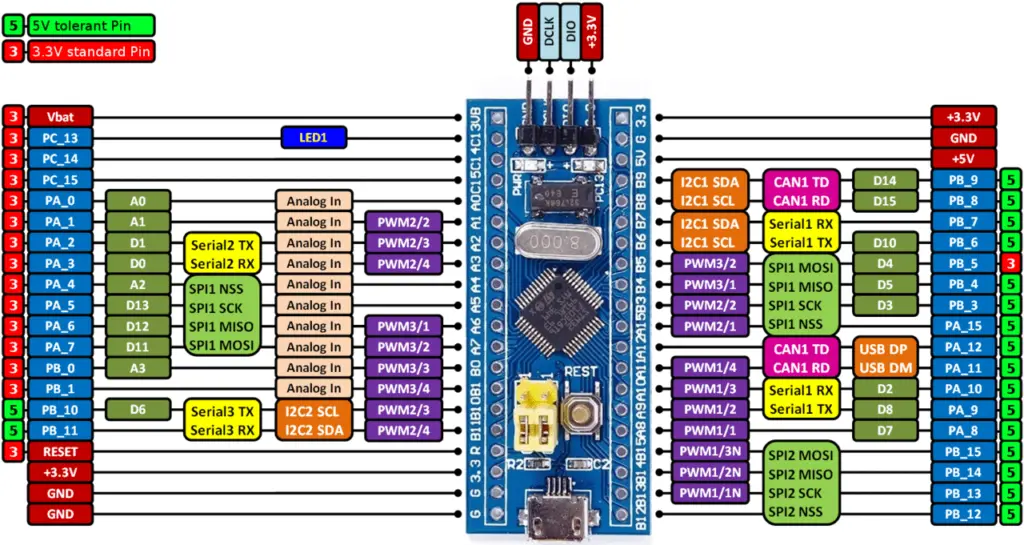
\includegraphics[width=0.80\textwidth]{assets/stm32_bluepill.png}
    \captionsetup{justification=raggedright}
    \caption*{Fonte: \figcite{STMBoardProductPage}}
    \label{fig:stm32Bluepill}
\end{figure}

Para a injeção de falhas será utilizado o depurador GDB em conjunto com uma ferramenta de depuração de hardware ST-LINK (\autoref{fig:stLink}), a comunicação do ST-LINK é feita via USB com o computador e via JTAG com o microcontrolador alvo, também será usado em conjunto uma IDE fornecida pelo mesmo fabricante, a STM32Cube IDE.

\begin{figure}[H]
    \centering
    \captionsetup{justification=centering}
    \caption{ST-LINK/V2}
    
\includegraphics[width=0.50\textwidth]{assets/st_link.png}
    \captionsetup{justification=raggedright}
    \caption*{Fonte: \figcite{STLinkProductPage}}
    \label{fig:stLink}
\end{figure}

\begin{figure}[H]
    \centering
    \captionsetup{justification=centering}
    \caption{ST-LINK/V2}
    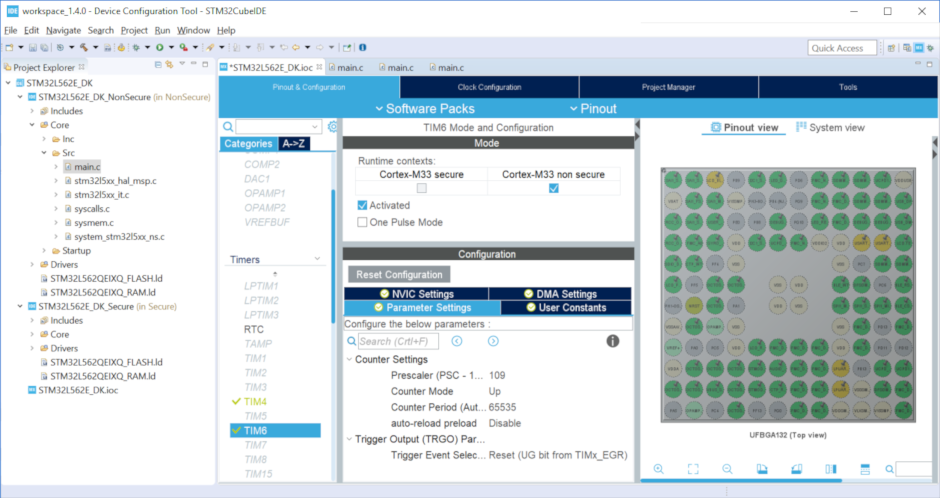
\includegraphics[width=0.80\textwidth]{assets/stmcube_ide.png}
    \captionsetup{justification=raggedright}
    \caption*{Fonte: \figcite{STMCubeProductPage}}
    \label{fig:stmCubeIDE}
\end{figure}

Durante a fase de desenvolvimento dos algoritmos será utilizado o QEMU juntamente com as ferramentas anteriormente citadas, assim como sanitizadores de memória e condições de corrida (ASan, TSan, UBSan) para auxiliar na detecção de erros mais cedo durante o desenvolvimento.

O sistema operacional de tempo real escolhido foi o FreeRTOS, por ser extensivamente testado e documentado e prover um escalonador totalmente preemptivo com um custo espacial relativamente pequeno, além disso, os contribuidores do FreeRTOS mantém uma lista grande de versões para diferentes arquiteturas e controladores, facilitando drasticamente o trabalho ao não ter que criar uma HAL do zero.

\subsection{Métodos}

Serão utilizadas as seguintes técnicas de tolerância à falhas implementadas em software: CRCs para mensagens, redundância modular, reexecução, sinal heartbeat e asserts. O detalhamento específico de cada técnica é abordado em maior detalhe na \autoref{subsec:algoritmos}.

Para a criação da análise, serão realizados testes com injeção lógica em hardware utilizando-se do ST-Link em combinação com um computador que emitirá os comandos para injeção via depurador, as falhas serão de natureza transiente e afetarão valores na memória (corrupção silenciosa) assim como nos registradores que não são de controle. A \autoref{fig:injecaoHardwareLogica} detalha de forma mais específica o fluxo de gerar uma falha. As combinações específicas de falhas e técnicas escolhidas são abordadas na \autoref{subsec:campanhaInjecao}.

\begin{figure}[H]
   \centering
   \captionsetup{justification=centering}
   \caption{Injeção lógica em hardware}
   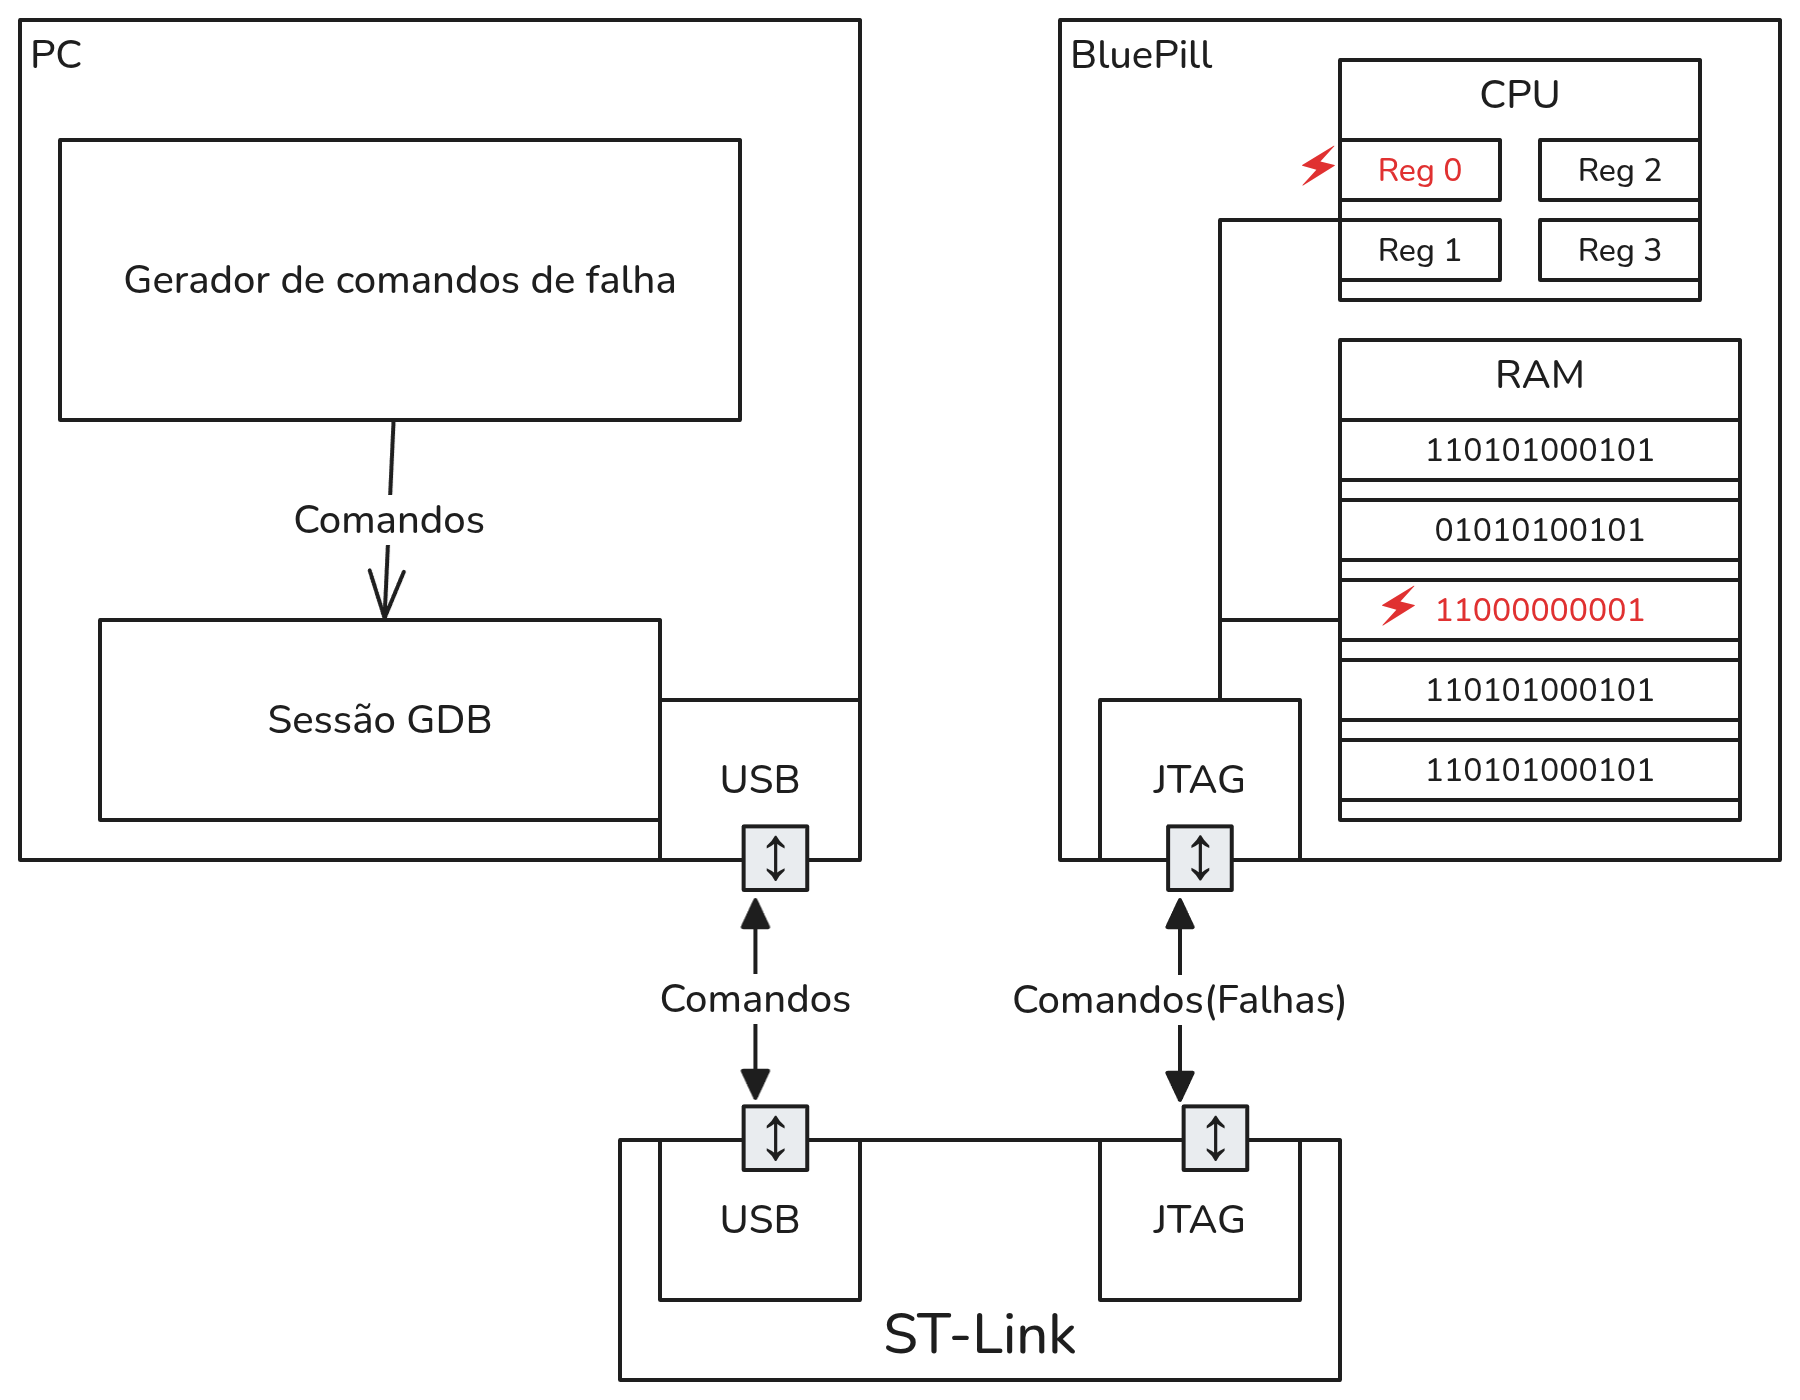
\includegraphics[width=0.90\textwidth]{assets/injecao_hardware.png}
   \captionsetup{justification=raggedright}
  \caption*{Fonte: Elaborada pelo autor}
   \label{fig:injecaoHardwareLogica}
\end{figure}

A coleta de métricas será realizada com os mecanismos de monitoramento do sistema FreeRTOS juntamente com contadores de incremento atômico, o tempo de execução das tarefas, seu espaço de memória utilizado e o número de falhas detectadas será armazenado em uma estrutura que residirá em um segmento de memória que é deliberadamente isento de falhas.

Com o objetivo de promover a reutilização de código e a abstração, será implementada uma interface que generaliza um objeto de tarefa. Considerando que um objeto que realiza despache dinâmico requer uma tabela de despacho virtual (V-Table), faz-se necessário adotar precauções adicionais, dado que a própria tabela pode estar sujeita a falhas. Para mitigar esse risco, será aplicada uma replicação simples dos ponteiros de função da V-Table, resultando em um custo adicional de duas comparações por chamada de método. A interação da interface com o resto do sistema é abordada em maior detalhe na \autoref{subsec:interface}.

\section{Análise de requisitos}
\label{sec:req}

\begin{quadro}[H]
    \centering
    \caption{Requisitos funcionais}
    \begin{tabular}{|p{0.125\textwidth}|p{0.8\textwidth}|}
        \hline
        \rowcolor[HTML]{C0C0C0}
        \textbf{Requisito} & \textbf{Descrição}  \\
        \hline
        
        \textbf{RF01} & Implementação de todos os algoritmos descritos na \autoref{subsec:algoritmos} \\ 
        \hline

        \textbf{RF02} & Criação, finalização e cancelamento de tarefas e recuperação de sua memória alocada \\
        \hline
        
        \textbf{RF03} & Configuração do mecanismo de tolerância, prioridade e prazo de execução da tarefa \\
        \hline

        \textbf{RF04} & Cumprimento do prazo estipulado no momento de criação da tarefa caso não exista presença de falhas \\
        \hline

        \textbf{RF05} & Detecção e reação à falhas de corrupção de memória \\
        \hline

        \textbf{RF06} & Detecção e reação à falhas de vencimento de prazo de execução \\
        \hline
        
        \textbf{RF07} & Monitoramento do número de falhas detectadas e violações de prazos  \\
        \hline
        
        \textbf{RF08} & Comunicação entre tarefas por uma fila com checagem dos pacotes \\
        \hline
    \end{tabular}
    \label{tab:rf}
\end{quadro}

\begin{quadro}[H]
    \centering
    \caption{Requisitos não funcionais}
    \begin{tabular}{|p{0.125\textwidth}|p{0.8\textwidth}|}
        \hline
        \rowcolor[HTML]{C0C0C0}
        \textbf{Requisito} & \textbf{Descrição}  \\
        \hline
        
        \textbf{RNF01} & O consumo de memória deve ser pré determinado em tempo de compilação ou na inicialização do sistema \\
        \hline
        
        \textbf{RNF02} & A interface deve ser construida sobre o escalonador preemptivo do FreeRTOS \\
        \hline

        \textbf{RNF03} & Deve ser compatível com arquitetura ARMv7M ou ARMv8M \\
        \hline

        \textbf{RNF04} & Implementação realizada em C++ (versão 20 ou acima) \\
        \hline
        
        \textbf{RNF05} & Código fonte da interface disponível sob licença permissiva (BSD3) \\
        \hline
    \end{tabular}
    \label{tab:rnf}
\end{quadro}

\subsection{Interface} \label{subsec:interface}

Para melhor generalizar o uso das técnicas, utiliza-se de uma abstração da estrutura de tarefa juntamente com um mecanismo de passagem de mensagens com detecção de erros.

Uma mensagem envelopa um pacote de dados qualquer para que possa ser enviado de forma assíncrona entre tarefas. Neste caso, o ordenamento dos campos é importante: o pacote precisa ser o último membro para serialização de estruturas de tamanho arbitrário, a distribuição dos campos na memória é demonstrada na \autoref{fig:messageStruct}. 

\begin{figure}[H]
    \centering
    \captionsetup{justification=centering}
    \caption{Layout de uma mensagem}
    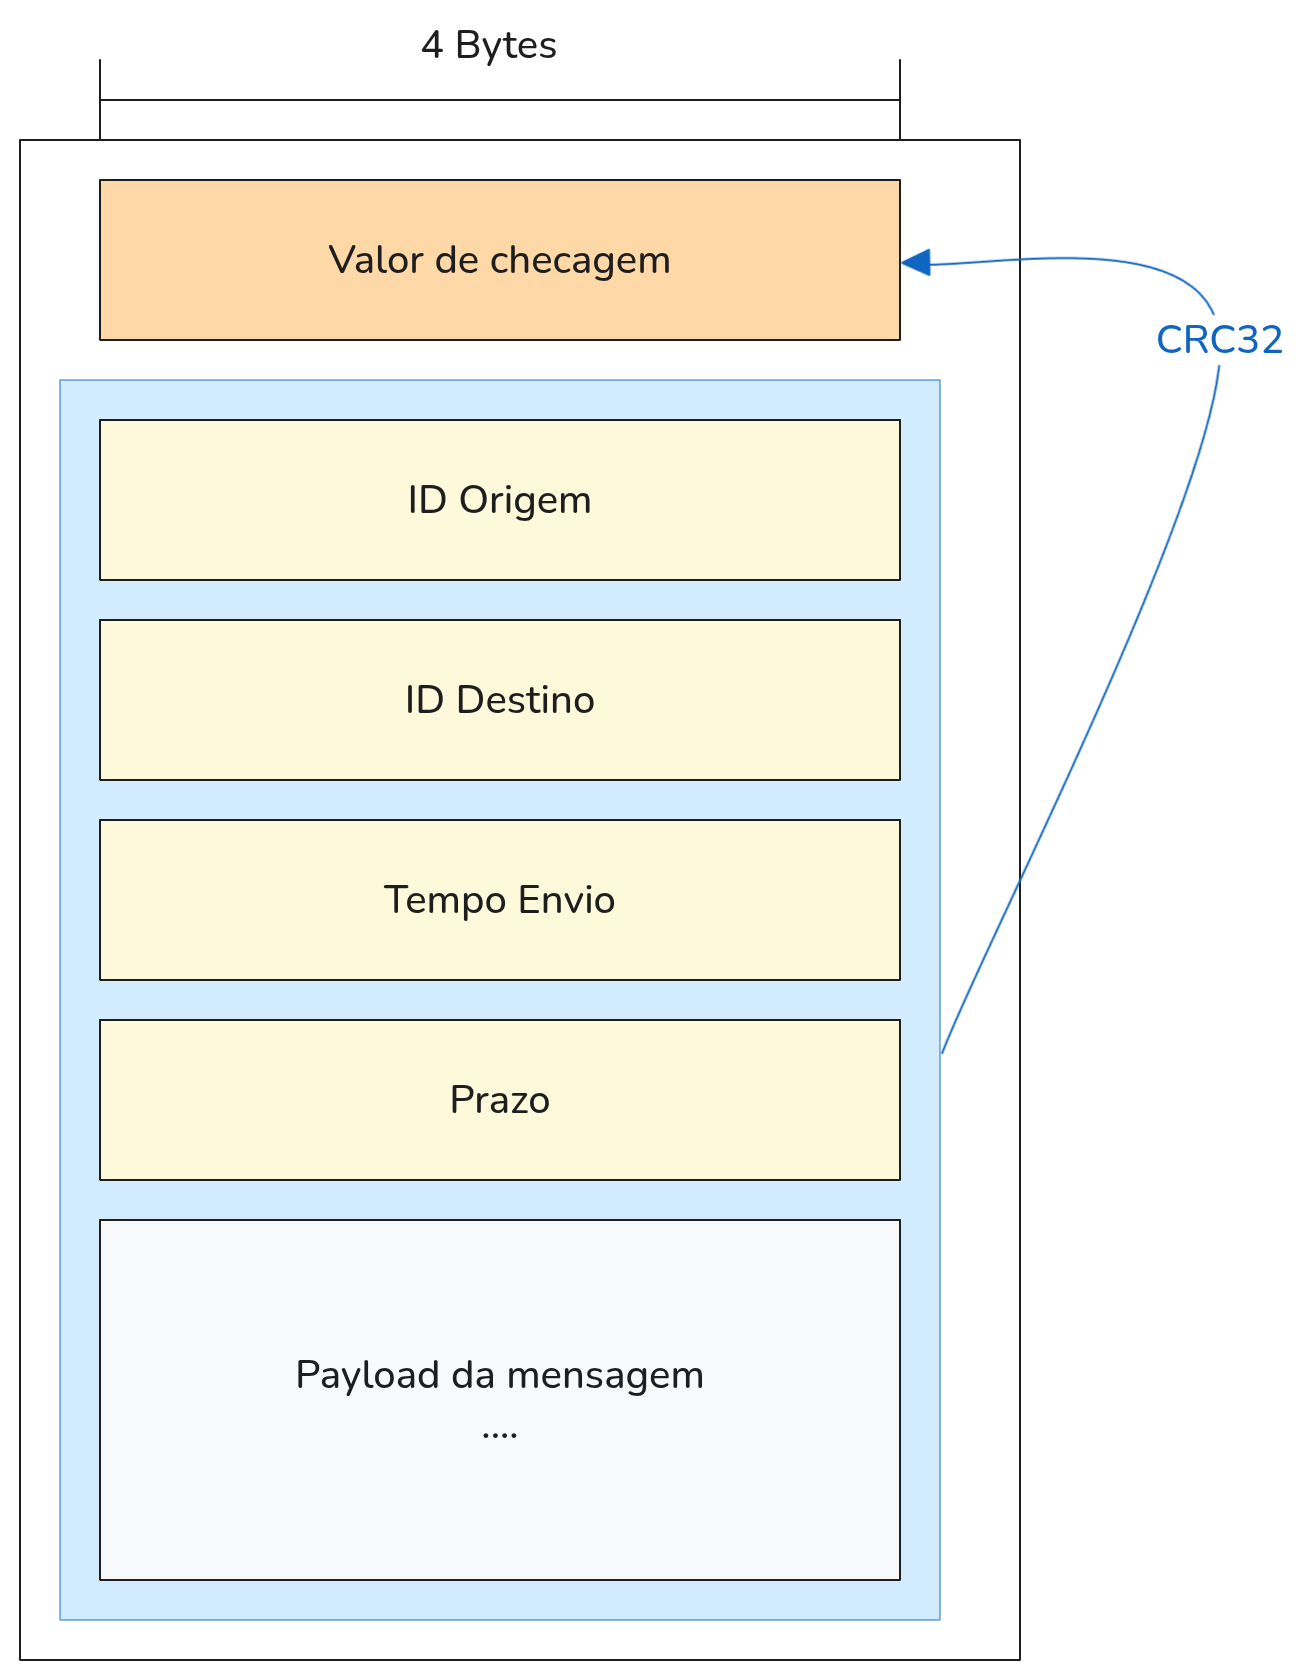
\includegraphics[width=0.60\textwidth]{assets/payload_layout.png}
    \captionsetup{justification=raggedright}
    \caption*{Fonte: Elaborada pelo autor}
    \label{fig:messageStruct}
\end{figure}

A tarefa é um objeto de interface que abstrai parte do estado utilizado pelo RTOS e provê métodos para sua inicialização, término e cancelamento. Uma tarefa possui um espaço de pilha dedicado, e uma V-Table que inclui os métodos providos para sua execução. A identificação da tarefa se dá pelo seu ID, que diretamente mapeia o recurso que encapsula o estado da tarefa no RTOS. O diagrama na \autoref{fig:bddTarefa} demonstra a relação de uma tarefa e os outros componentes do sistema.

\begin{figure}[H]
    \centering
    \captionsetup{justification=centering}
    \caption{Objeto que implementa a interface de Tarefa}
    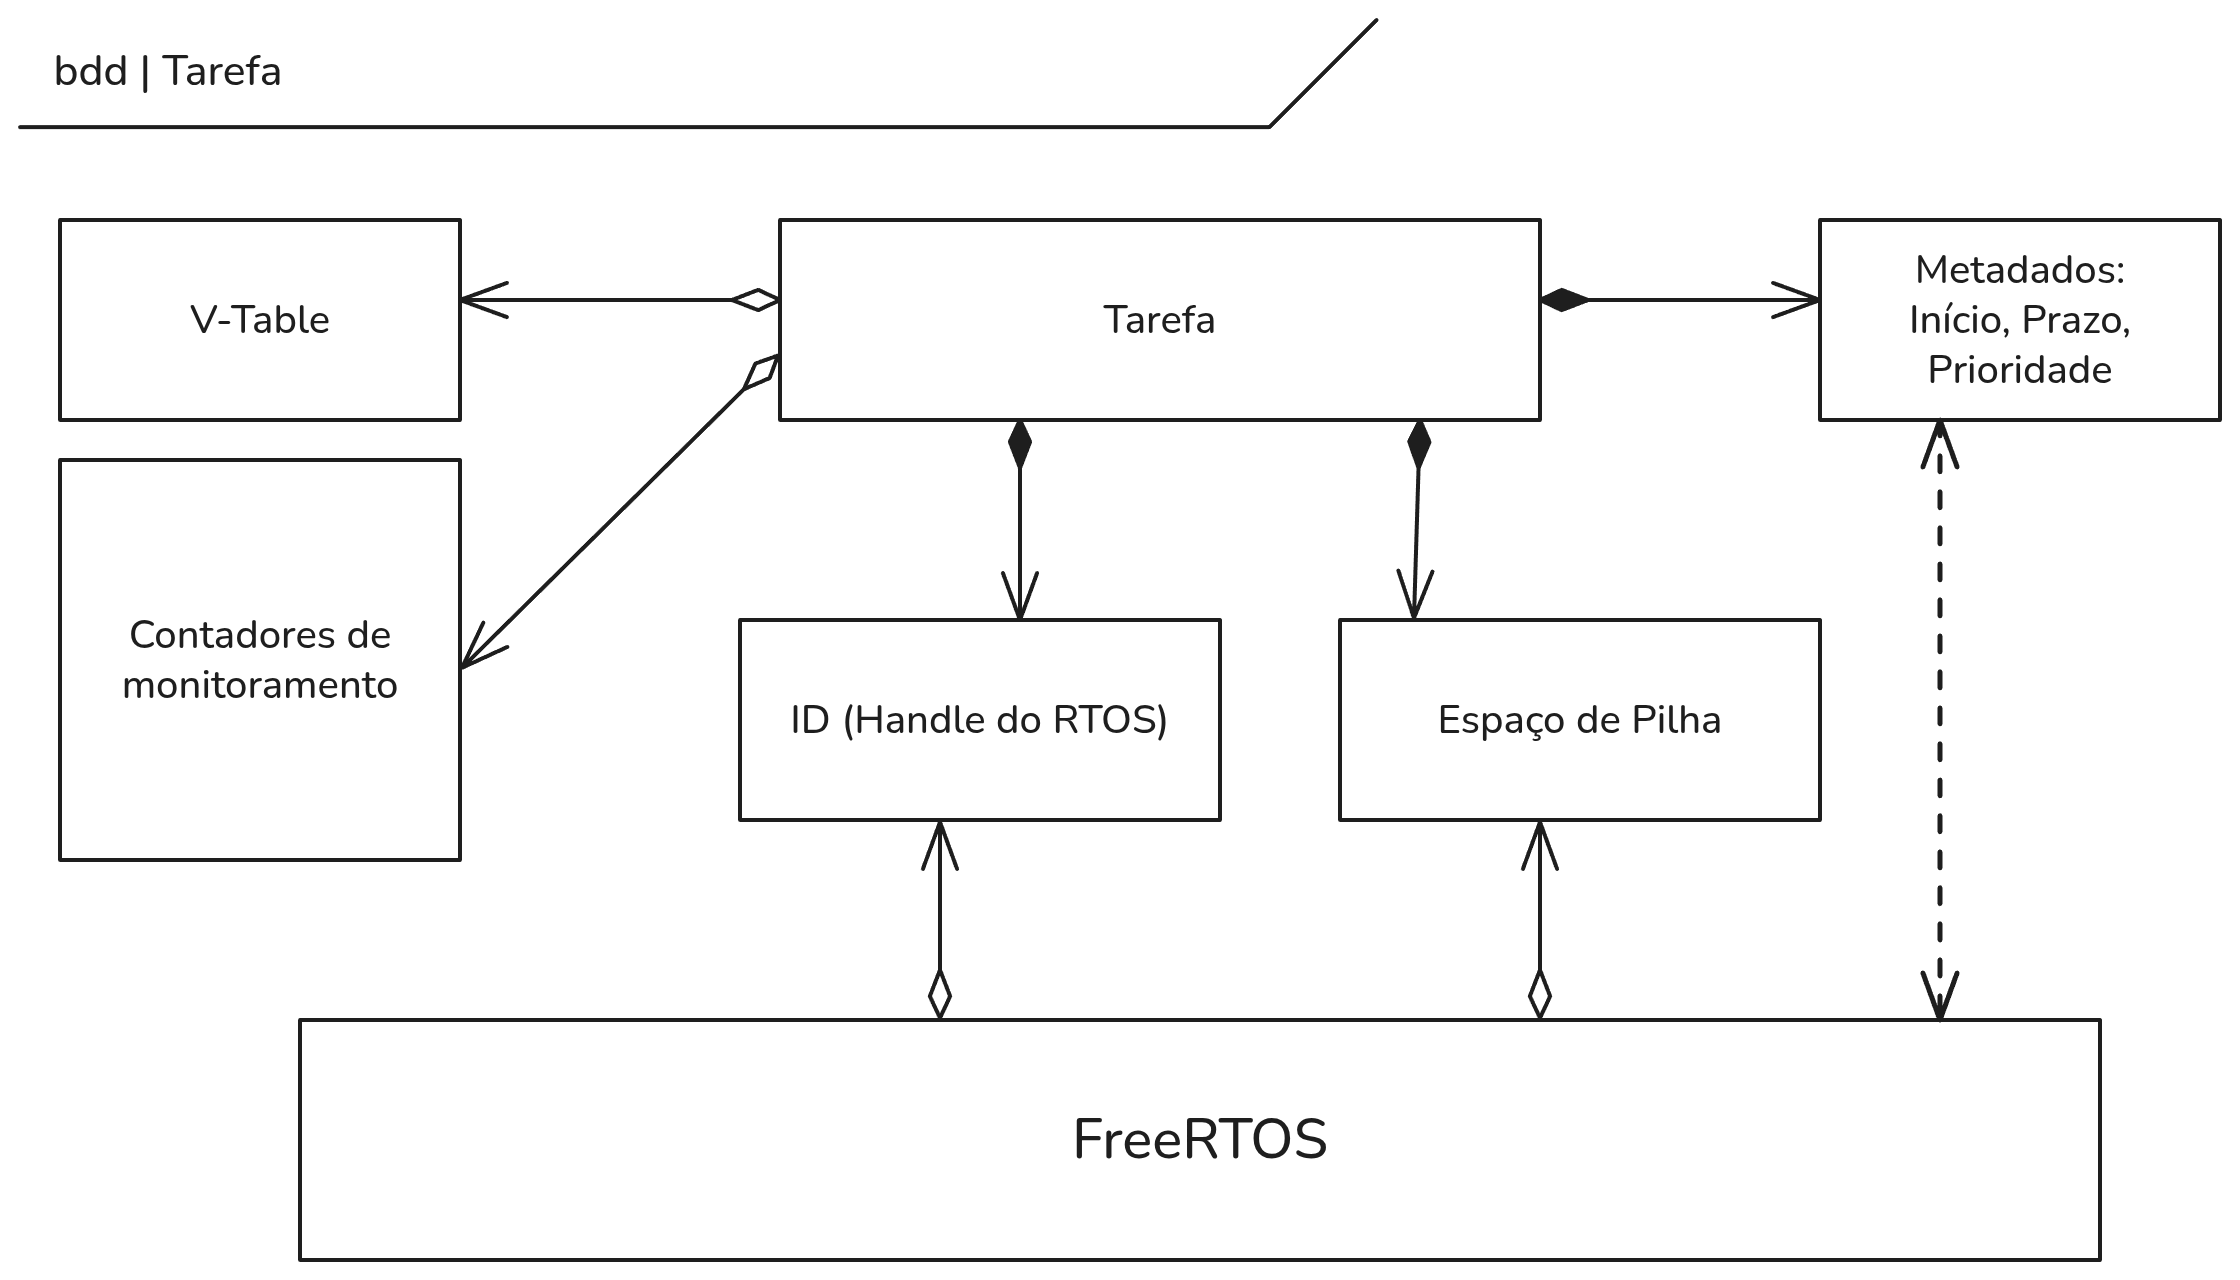
\includegraphics[width=0.90\textwidth]{assets/task_bdd.png}
    \captionsetup{justification=raggedright}
    \caption*{Fonte: Elaborada pelo autor}
    \label{fig:bddTarefa}
\end{figure}

A \autoref{fig:bddTarefa} omite a replicação da V-Table por clareza visual, mas antes da invocação de qualquer método da V-Table, será feito uma comparação adicional com outras duas tabelas redundantes para detectar corrupções na própria tabela durante a indireção por ponteiro de função.

\subsection{Algoritmos e Técnicas} \label{subsec:algoritmos}

Para a implementação da funcionalidade de tolerância à falhas, algumas das técnicas abordadas no \autoref{cap:fund} serão utilizadas. O detalhamento sobre a implementação será abordado nesta seção.

\subsubsection{CRC: Cyclic Redundancy Check}

Será implementado o CRC-32C, que já é aplicado em sistemas de arquivos como o Btrfs e o ext4, assim como em protocolos de rede como iSCSI e SCTP. Seu Polinômio geradador $P$ é:

\begin{equation}
	\begin{split}
		P = & x^{32} + x^{28} + x^{27} + x^{26} + x^{25} + x^{23} + x^{22} + x^{20} \\
	        & + x^{19} + x^{18} + x^{14} + x^{13} + x^{11} + x^{10} + x^{9} + x^{8} + x^{6} + 1
	\end{split}
\end{equation}
\addEquacao{Polinômio CRC-32C}{5}


\subsubsection{Redundância Modular}

Para a aplicação da redundância modular, neste caso a redundância modular tripla, será feito a replicação concorrente da tarefa, cada tarefa possui um espaço de pilha próprio e são escalonadas de forma convencional pelo FreeRTOS. O corpo das tarefas não é replicado, e continua como parte de memória para apenas leitura e execução, um exemplo da relação de réplicas de tarefas executando em relação ao resto do sistema pode ser observado na \autoref{fig:bddTMR}.

\begin{figure}[H]
    \centering
    \captionsetup{justification=centering}
    \caption{Diagrama de bloco de Redundância modular}
    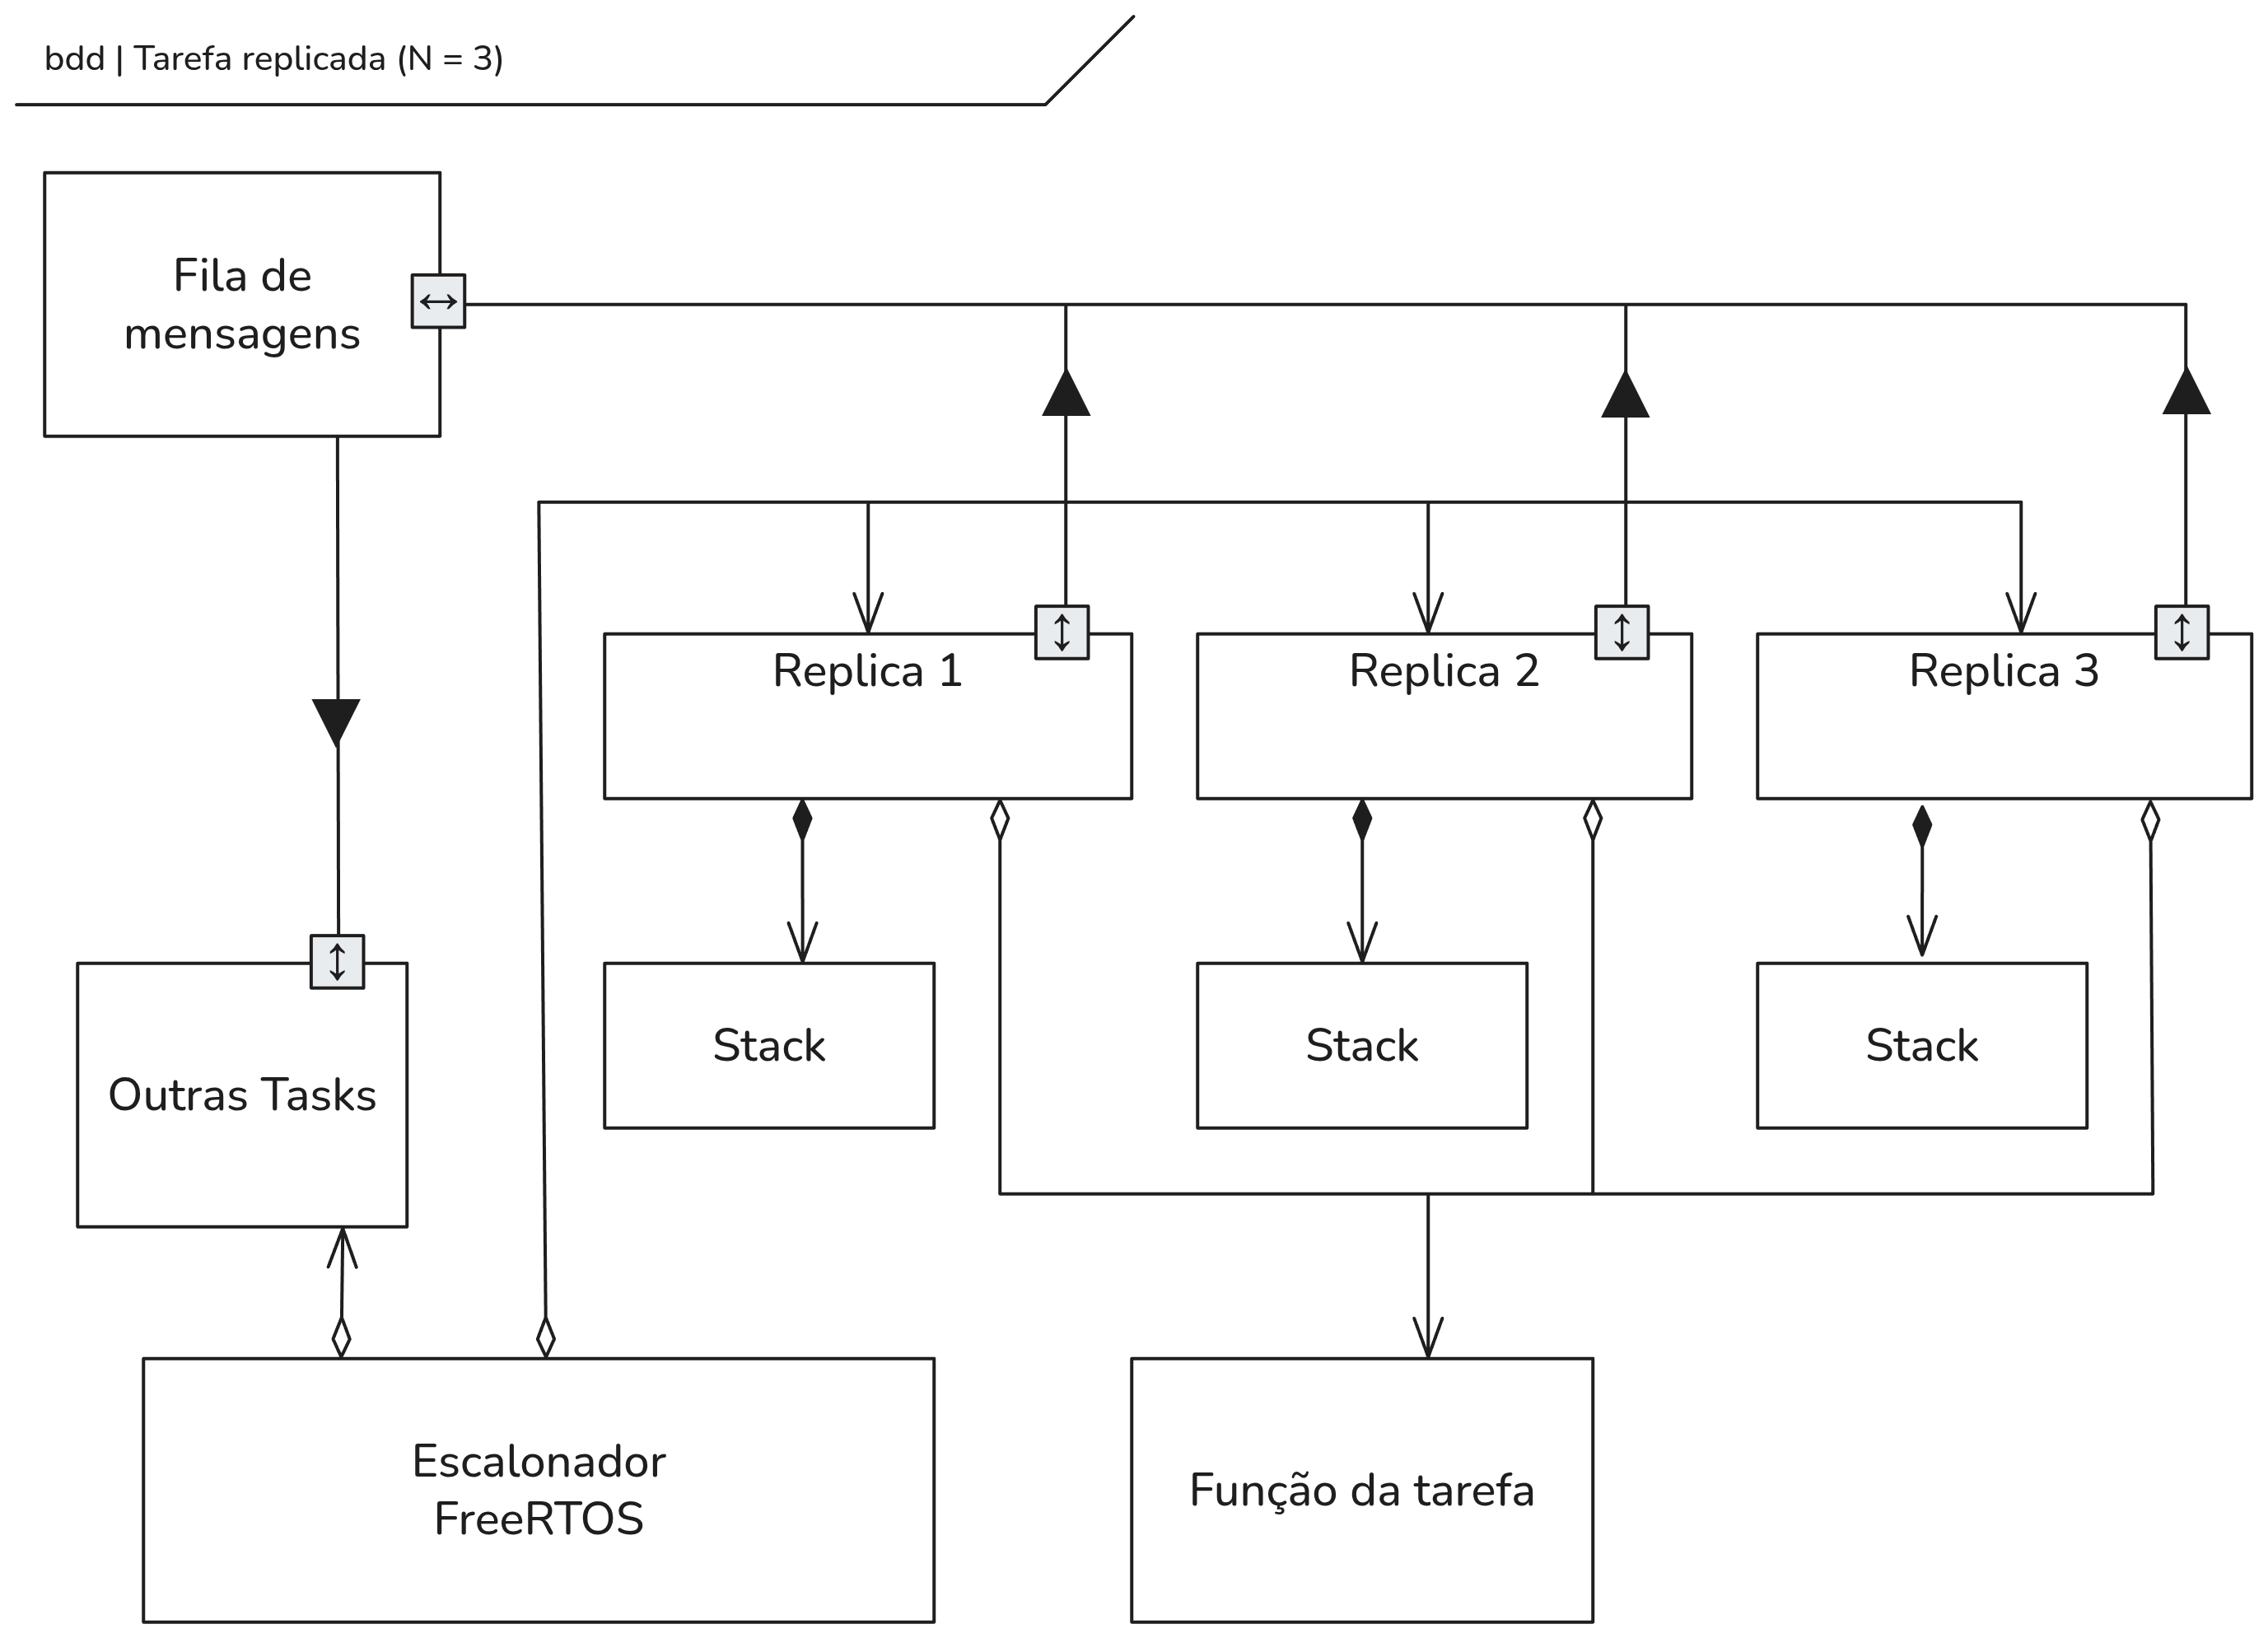
\includegraphics[width=0.975\textwidth]{assets/tmr_bdd.png}
    \captionsetup{justification=raggedright}
    \caption*{Fonte: Elaborada pelo autor}
    \label{fig:bddTMR}
\end{figure}

\subsubsection{Reexecução}

A implementação de tarefas com reexecução é baseada no uso de execuções consecutivas que reutilizam do mesmo espaço de pilha, uma tarefa pode ser sempre reexecutada $N$ vezes, servindo um propósito similar à técnica de redundância, ou executada \textit{até} $N$ vezes, encerrando a execução imediatamente após não encontrar nenhuma falha. Para os propósitos deste trabalho, será utilizada a segunda técnica, pois permite mais oportunidade para o escalonador encaixar trabalho no tempo ocioso, e também por ser um exemplo mais bem estudado na fundamentação teórica deste trabalho por Isosimov et. al.

Assumindo $N = 3$, o diagrama na \autoref{fig:stateReexec} descreve uma máquina de estado finito para a execução de uma tarefa com reexecução, espera-se que o caso médio seja a execução diretamente para um estado correto. Para a criação de uma condição de transparência, o prazo da tarefa deve ser o pior caso possível de $N$ execuções.

\begin{figure}[H]
    \centering
    \captionsetup{justification=centering}
    \caption{Estados de uma reexecução}
    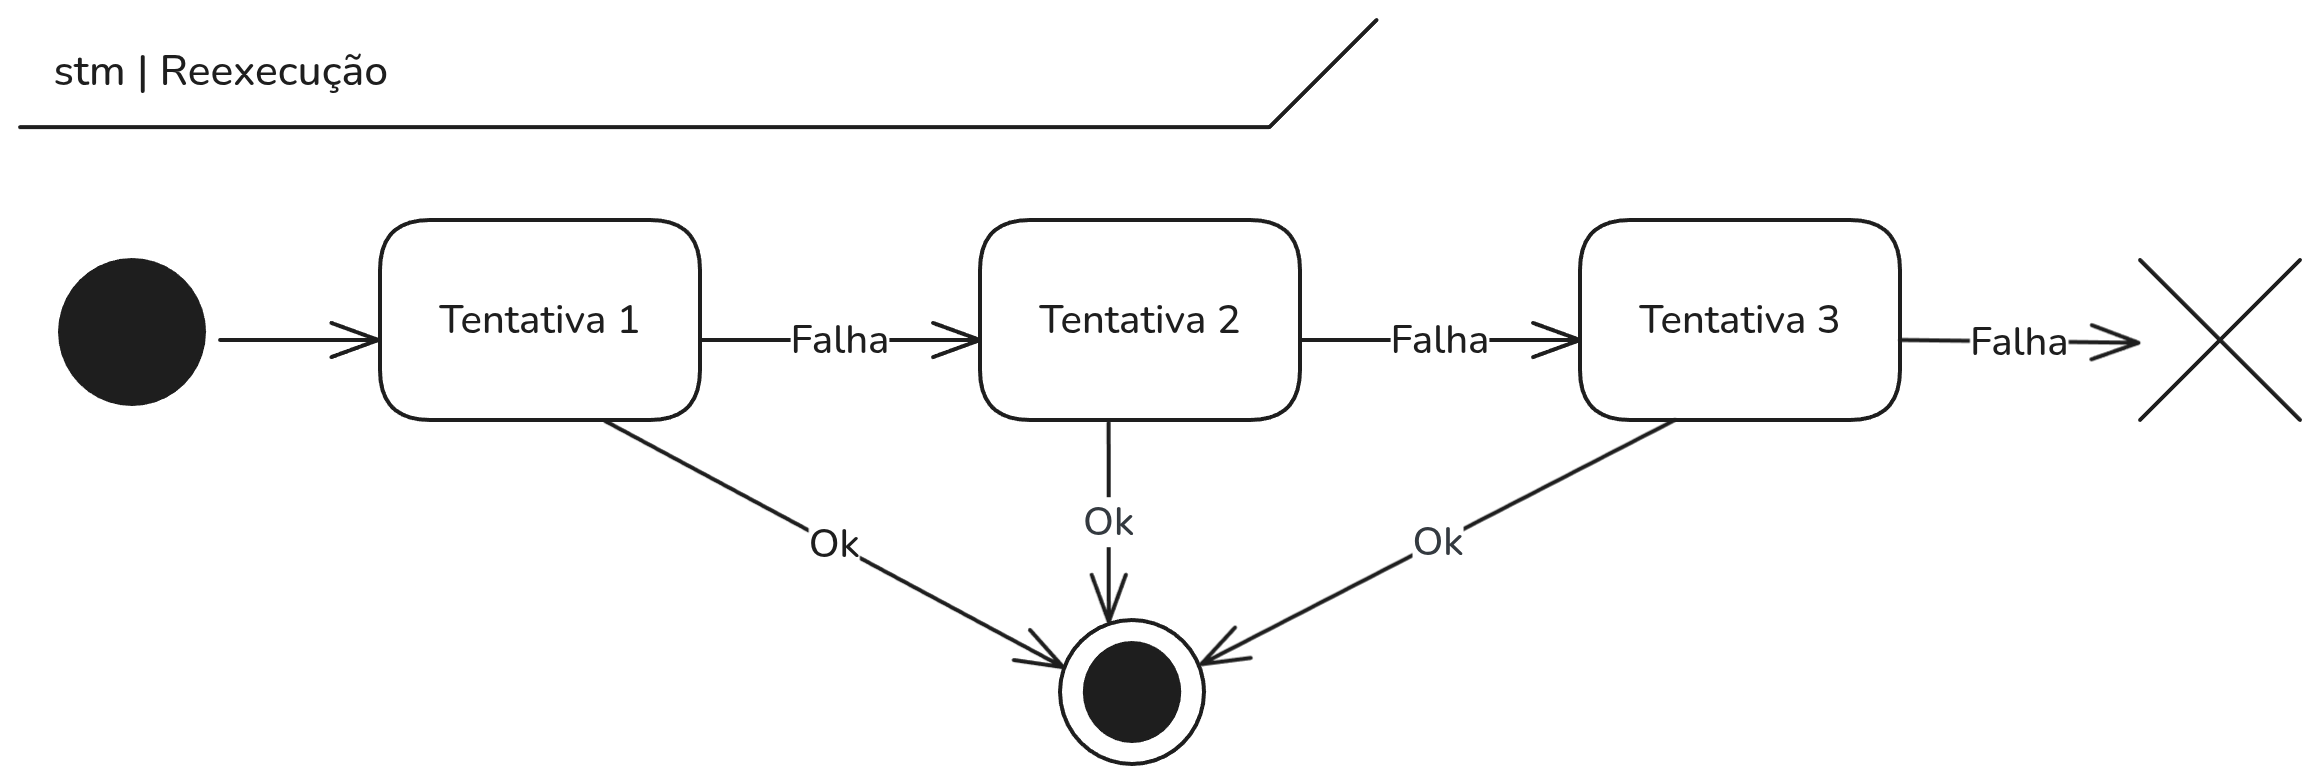
\includegraphics[width=0.975\textwidth]{assets/state_reexec.png}
    \captionsetup{justification=raggedright}
    \caption*{Fonte: Elaborada pelo autor}
    \label{fig:stateReexec}
\end{figure}

\subsubsection{Sinal Heartbeat}

Para a implementação dos sinais de heartbeat será utilizado uma tarefa que servirá como um monitor que associa os IDs de outras tarefas com um timer de sinal, o sinal será propagado com escrita atômica de um número e o temporizador do sistema no momento da escrita, se houver uma violação do prazo combinado na criação da tarefa e o prazo apresentado, é considerado que ocorreu uma falha. Este fluxo é visualmente representado na \autoref{fig:heartbeatAdv}. Essa técnica pode ser utilizada para cancelar tarefas presas no caso de replicação assim como iniciar uma reexecução antecipada.

\begin{figure}[H]
    \centering
    \captionsetup{justification=centering}
    \caption{Estados de uma reexecução}
    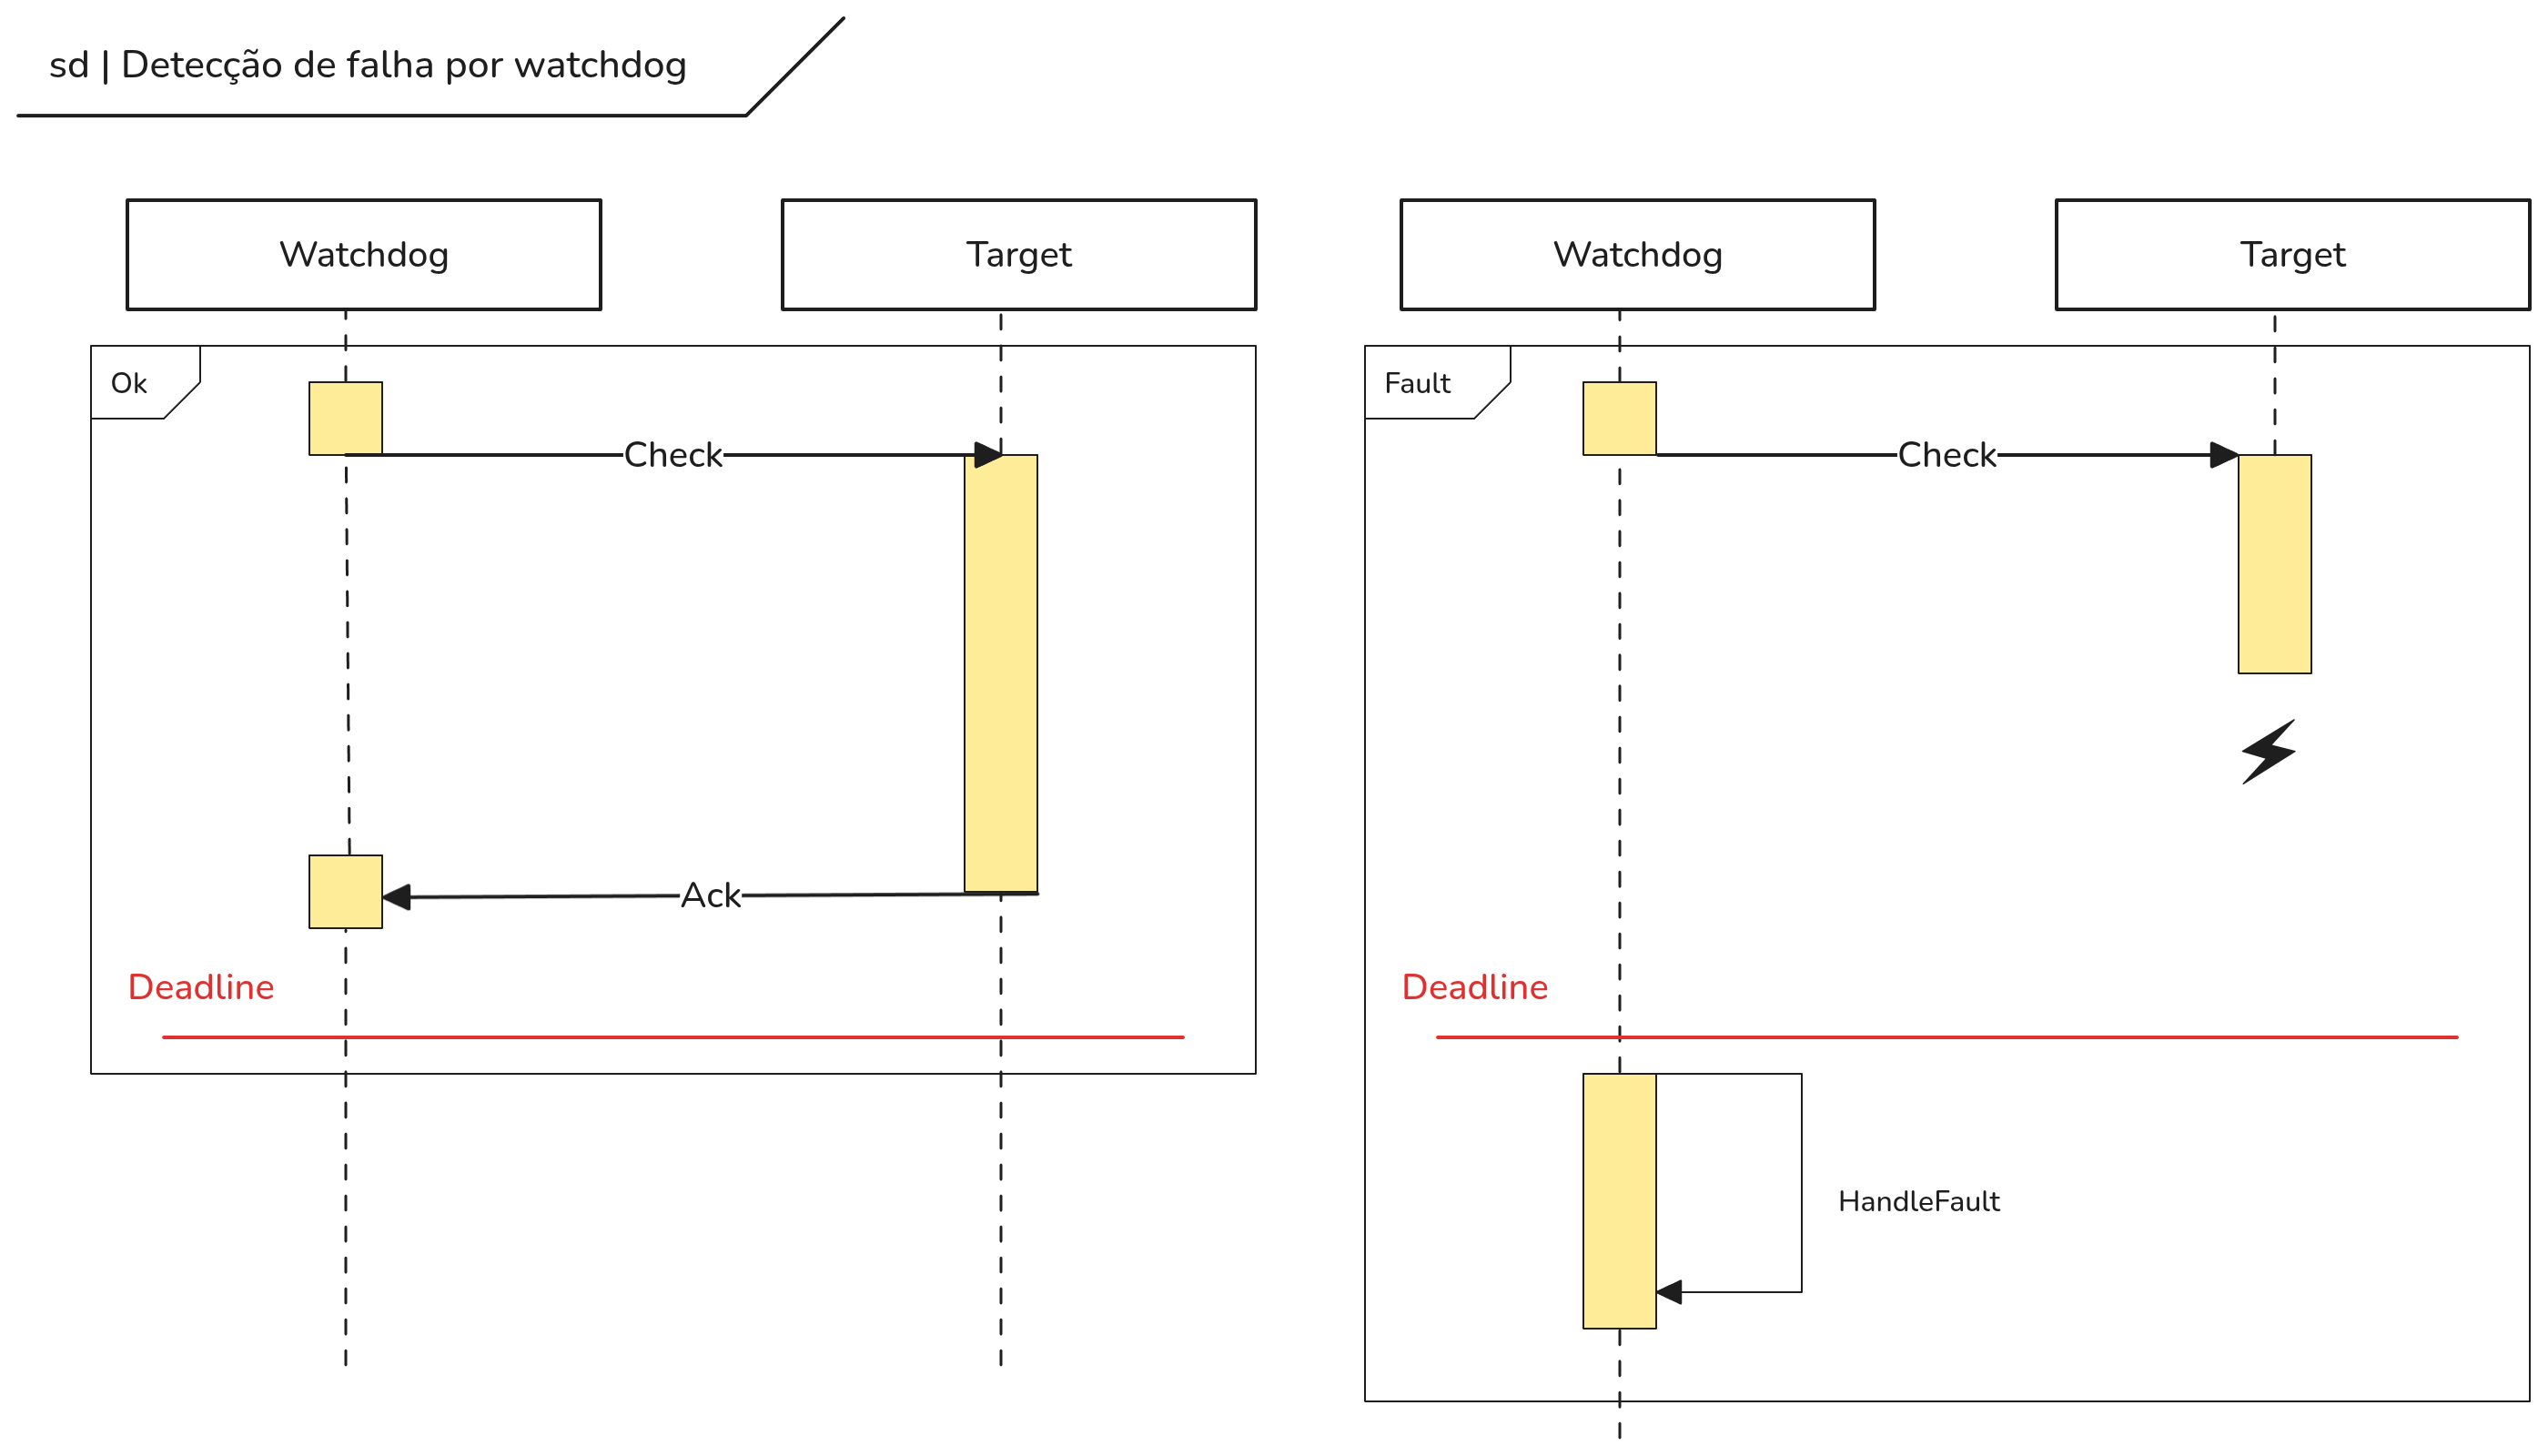
\includegraphics[width=0.975\textwidth]{assets/heartbeat_signal.png} %TODO: change to better image
    \captionsetup{justification=raggedright}
    \caption*{Fonte: Elaborada pelo autor}
    \label{fig:heartbeatAdv}
\end{figure}

\subsubsection{Asserts}

Asserts serão utilizados para verificar invariantes, qualquer quebra de contrato de função ou invariante que é coberta com um assert deve resultar em uma falha.

\section{Plano de Verificação}

Para a validação dos algoritmos e técnicas utilizadas(\textbf{RF01}, \textbf{RF08}) será feito uma série de testes unitários e de integração, para garantir que as técnicas estejam ao menos corretamente implementadas antes de realizar qualquer tipo de medição.

A validação da detecção de falhas e vencimento de prazos (\textbf{RC05}, \textbf{RF07}, \textbf{RF06}) serão preliminarmente testadas com injeção lógica em software utilizando o emulador QEMU com a mesma arquitetura de processador executando o sistema FreeRTOS e será validado definitivamente durante o teste com injeção lógica em hardware. A capacidade de criar, destruir e cancelar tarefas (\textbf{RF02}) é um pré-requisito e será verificada com um simples teste ponta a ponta. Importante notar que a priorização de tarefas baseadas em seu número de prioridade já é implementada pelo próprio FreeRTOS.

Como o produto final do trabalho requer uma análise de resiliência e do custo das técnicas, a seção seguinte aborda a campanha de injeção utilizada, que será aplicada com método lógico em hardware para a análise final.

\subsection{Campanha de Injeção de Falhas} \label{subsec:campanhaInjecao}


\section{Análise de Riscos} \label{sec:analiseRiscos}

O trabalho é de risco baixo, dado que constrói em cima de fundações técnicas previamente exploradas, porém dentro dos principais riscos que possam alterar ou causar problemas durante a produção da análise encontram-se:

\begin{quadro}[H]
    \centering
    \caption{Análise de riscos}
    \begin{tabular}{|p{0.20\textwidth}|p{0.150\textwidth}|p{0.10\textwidth}|p{0.20\textwidth}|p{0.20\textwidth}|}
        \hline
        \rowcolor[HTML]{C0C0C0}
        \textbf{Risco} & \textbf{Probabilidade} & \textbf{Impacto} & \textbf{Gatilho} & \textbf{Mitigação} \\
        \hline

        Funcionalidades e API do RTOS é incompatível com a interface proposta pelo trabalho &  Baixo & Alto & Implementar interface no RTOS & Utilizar outro RTOS, modificar o FreeRTOS, adaptar a interface \\
        \hline

        Problemas para injetar falhas com depurador em hardware & Baixa & Alto & Realizar injeção no microcontrolador & Utilizar de outro depurador, depender de falhas lógicas em software como última alternativa \\
        \hline

        Não conseguir coletar métricas de performance com profiler do FreeRTOS & Baixa & Médio & Teste em microcontrolador ou ambiente virtualizado & Inserir pontos de medição manualmente \\
        \hline

    \end{tabular}
    \label{tab:riscos}
\end{quadro}


% 04/07
% Refazer consideracoes finais
% Falar de tempo real no visão geral
% 05/07
% Ler o trabalho da Nicole

% COlocar como trabalho relacionado no lugar do de analise de fluxo la

